\chapter{Introduction}\label{chap:introduction}

\section{Sustainability}\label{sec:sustainability}
In 2015, the notion of \gls{sustainability} was defined by a set of 17 distinct goals by the UN \cite{UN_sustain}, called \acrfullpl{sdg}. Each goal was defined by a subset of different targets, aiming to define a successful completion of this goal. To evaluate the contribution of this work, the chosen research subject is mapped to specific goals and the concrete targets in section \ref{subsec:sustainabilityGoals}. The tangible legal frameworks, that are implemented in Germany are discussed in section \ref{subsec:nationalGoals}.

\begin{figure}[!h]
	\centering
	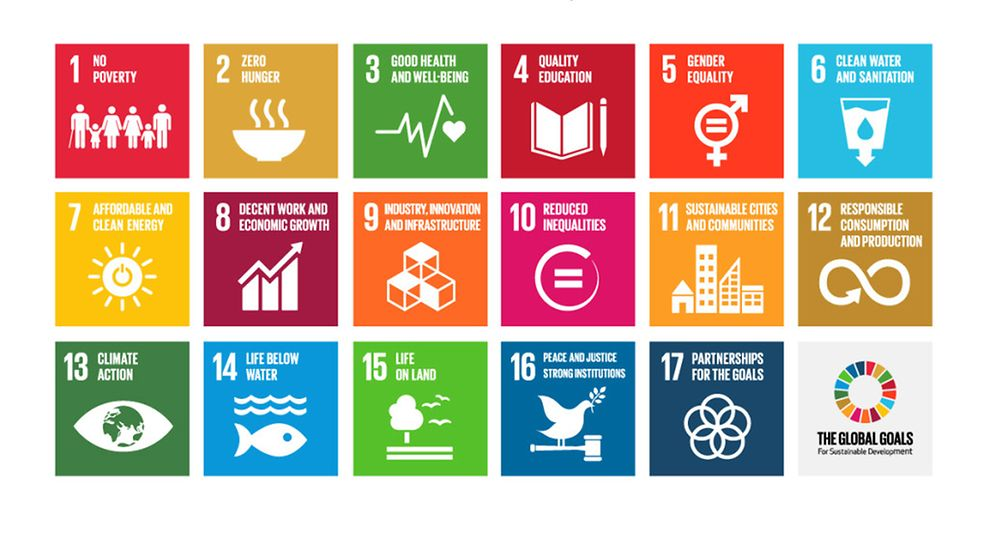
\includegraphics[width=\linewidth]{images/kacheln-the-global-goals.jpg}
	\caption{Overview of \acrfullpl{sdg} numbered from 1 to 17, adapted from The 2030 Agenda by Bundesregierung Deutschland, 2022 \cite{pic:eu_goals}.}
	\label{fig:sustainGoals}
\end{figure}


\subsection{Sustainability Targets}\label{subsec:sustainabilityGoals}
In the discussion on sustainability, the service sector is involved in almost all goals listed by the EU. The numbering of all specified goals can be seen in figure \ref{fig:sustainGoals} and are listed as follows:\\
\begin{tabular*}{\textwidth}{lclc}
	\hline
	1 & No Poverty & 9 & Industry, Innovation And Infrastructure\\
	2 & Zero Hunger & 10 & Reduced Inequalities\\
	3 & Good Health and Well-Being & 11 & Sustainable Cities \& Communities\\
	4 & Quality Education &	12 & Responsible Consumption \& Production\\
	5 & Gender Equality & 13 & Climate Action\\
	6 & Clean Water \& Sanitation & 14 & Life Below Water\\
	7 & Affordable \& Clean Energy & 15 & Life On Land\\
	8 & Decent Work \& Economic Growth & 16 & Peace \& Justice, Strong Institutions\\
	\hline
\end{tabular*}
\vskip
While providing good paying jobs through less physically intensive work, and easily accessible education, coordination services, IT and office work provides positive influences to goals regarding economic prosperity, equality and innovation (1, 2, 4, 5, 8, 9 and 10). As such the positive influences of work in this sector should be sustained as much as possible. On the other hand, service sector corporations can actively create challenges to physical and mental well being, manifested in \gls{sdg} number 3, as IT occupations are often sedentary and mentally demanding. Goals regarding Sustainable consumption, city development, institutional regulation and clean environment needs (\glspl{sdg} 6, 11, 12 and 16) can be at odds with the needs of the IT sector, due to the push to urbanization by office jobs, the variety of supply needs in modern offices. While mostly being neutral to almost all other goals, after the initial challenges are met, the sustainability can be threatened with respect to affordable and clean energy (goal 7) simply due to the existence of fully supplied offices in a developed country. Energy demands due to production, operation and demolition are a constant byproduct of economic activity in the service and IT sector. In order to facilitate the positives of office work, our goal should be to minimize negative effects in these specific other areas. Energy efficiency is an adequate tool to mitigate parts of the damages ensued due to office economy. However, to find effective ways to curb electricity consumption in all areas, a solid knowledge foundation is key, to compare and evaluate problems and solutions in the field. On the side of energy generation it is important to analyze the technical and political framework to energy availability, and the respective environmental costs.  
\begin{figure}
        \centering
        \begin{tabular}{ccc}
        	\subgraphics{GOAL_7_TARGET_7.3.png}{}&
        	\subgraphics{GOAL_9_TARGET_9.C.png}{}&
        	\subgraphics{GOAL_11_TARGET_11.6.png}{}\\
        	\subgraphics{GOAL_12_TARGET_12.6.png}{}&
        	\subgraphics{GOAL_12_TARGET_12.8.png}{}&
        	\subgraphics{GOAL_13_TARGET_13.3.png}{}
        \end{tabular}
        \caption{Collection of targets concerned by energy efficiency adapted from Global Goals, 2022 via 'https://www.globalgoals.org/resources/'.}
        \label{fig:targets}
\end{figure}  

\subsection{National Goal Implementations}\label{subsec:nationalGoals}
As a member of the European Union, the german government for the first time enacted in 2019 the respective goals into national policy with an agenda tackling every sustainability goal with the following points:\pagebreak
\begin{itemize}
	\item Human well-being and capabilities, social justice (SDGs 3, 4, 5, 8, 9, 10)
	\item Climate action and energy transition (SDGs 7, 13)
	\item Circular economy (SDGs 8, 9, 12)
	\item Sustainable building and transport (SDGs 7, 8, 9, 11, 12, 13)
	\item Sustainable agricultural and food systems (SDGs 2, 3, 8, 12, 13)
	\item A pollutant-free environment (SDGs 6, 8, 9, 14, 15)
\end{itemize}
While adapting the goals of the European Union, the specific implementation is similarly vague, in most cases. In terms of greenhouse gas emission, these goals were defined to incorporate a reduction of emissions by 65\% until 2030 compared to the level of 1990, up to a final CO$_2$ neutrality by 2045 \cite{german_goals}.
\newpage
\section{Power Consumption as a Contributor}\label{sec:powerConsumption}
From publications by the Umweltbundesamt, around 84\% of CO$_2$ equivalent emissions are produced due to emissions regarding energy and heat generation. While the total amount of CO$_2$ emissions are receding, this partition remains almost constant \cite{co2_contrib}. Therefore in order to fulfill CO$_2$ neutrality by the year 2045, more than 80\% of the problem stems from meeting any kind of energy demands. As part of the Federal Climate Change Act of 2021, the legal binding achievement of emission neutrality was finalized.
The legal goal and methodology is posted as "Climate neutrality of the federal administration is to be achieved, in particular, through
energy savings, through the efficient provision, conversion, use and storage of energy and
efficient use of renewable energy sources and the selection of the most climatefriendly modes of transport" \cite{fccl}. While setting clear milestones in a specific time frame, the legislation only sets out a very vague set of interventions. In light of achieving these goals, this work sets out to investigate possible contributions available in the context of energy consumption in office environments. The three objectives are defined as:
\begin{itemize}
	\item[1.] Generation of a robust and reliable energy consumption data set.
	\item[2.] Estimating the direct impact of consumed electricity on CO$_2$ footprint.
	\item[3.] Use well defined \acrfullpl{kpi} to identify optimization potential in energy consumption.
\end{itemize}
The section \ref{chap:relatedworks} highlights related works intersecting with these three research aspects and the office environment.
